\section{Глава 3. Алгоритм оценки фазы и частоты ШПС сигнала на основе АР-модели на фоне интерференции}

\subsection{Оценка фазы ПСП в ШПС}
\label{sec_dma_real}
Для использования параметрического метода оценки частоты необходимо восстановить гармоническую форму сигнала. Для этого
нужно получить оценку фазы ПСП и произвести повторную модуляцию входной смеси. Получить оценку фазы ПСП не прибегая к перебору по частоте,
позволяет алгоритм Delay and Multiply Approach (DMA). Данный алгоритм был представлен в статье и книге американского ученого Дж.Цуя \cite{lin_dma, tsui}

%Запишем входной сигнал в двух квадратурном виде:
%\begin{center}
%\begin{equation}
%	\label{eq:dma_lo_signal}
%	s(t)=C(t)e^{j2{\pi}f_{0}t}
%\end{equation}
%\end{center}
%где $C(t)$ - амплитуда, а $f_{0}$- частота несущей сигнала.
%
%Если входящий комплексный сигнал имеет задержку $\tau$, то данный сигнал будет описываться формулой: 
%\begin{center}
%\begin{equation}
%	\label{eq:dma_signal}
%	s(t-\tau)=C(t-\tau)e^{j2{\pi}f_{0}(t-\tau)}
%\end{equation}
%\end{center}
%
%Получим новый сигнал путем умножения \ref{eq:dma_lo_signal} и \ref{eq:dma_signal}:
%\begin{center}
%\begin{eqnarray}
%	s_{n}(t) & = & s(t)s(t-\tau)^{*}=\nonumber \\
%	 & = & C(t)C(t-\tau)e^{j2\pi f_{0}t}e^{j2\pi f(t-\tau)}=\label{eq:dma}\\
%	 & = & C(t)C(t-\tau)e^{j2\pi f_{0}\tau}\nonumber 
%\end{eqnarray}
%
%\par\end{center}
%
%Из формулы \ref{eq:dma} видно, что полученный сигнал не зависит от
%задержки $\tau$. Остается найти фазу ПСП. Референсный сигнал
%$C(t)C(t-\tau)$ используется для корреляции с новым кодом, который
%получен по формуле \ref{eq:dma} - умножением принятого сигнала и его задержанной
%копии. Когда фаза ПСП найдена, поиск сводится к одномерному поиску
%частоты. Данный метод позволяет уменьшить количество вычислений, путем
%сведения задачи поиска в двух измерения: по фазе кода и частоте; к
%задаче поиска только по частоте. Этот метод позволяет существенно
%сэкономить вычислительные ресурсы при обнаружении сигнала заданного
%спутника, но, вместе с тем, операция умножения повышает шум в процессе.
%
%\subparagraph{Aнализ изменения ОСШ при использовании алгоритма DMA}
%\label{sssec:dma_noise}
%
%Воспользуемся математическим аппаратом теории вероятностей. Необходимый математический аппарат
%рассмотрен в \cite{ventcel}, для более подробного изучения можно ознакомиться с \cite{feller}.
%Для упрощения можно принять, что в эфире только 1 сигнал (интерференция будет создавать окрашенный шум).
%
%Добавим в формулу \ref{eq:dma} АБГШ:
%\begin{center}
%\begin{eqnarray}
%	\label{eq:dma_general}
%	x_{n}(t) & = & (s(t)+n_{1}(t))(s(t-\tau)+n_{2}(t))^{*}=\nonumber \\
%	 & = & C(t)C(t-\tau)e^{j2{\pi}f_{0}{\tau}}+\nonumber \\
%	 & + & C(t)e^{j2{\pi}f_{0}t}n_{2}(t)+\label{eq:dma_noise_1}\\
%	 & + & C(t-\tau)e^{j2{\pi}f_{0}(t-\tau)}n_{1}(t)+\nonumber \\
%	 & + & n(t)^{2}\nonumber 
%\end{eqnarray}
%\end{center}
%где $C(t)C(t-\tau)e^{j2{\pi}f_{0}{\tau}}$ - новая ПСП, умноженная на константу, а
%$C(t)e^{j2{\pi}f_{0}t}n_{2}(t)+C(t-\tau)e^{j2{\pi}f_{0}(t-\tau)}n_{1}(t) + n(t)^{2}$ -
%шумовая компонента.
%
%Свойства дисперсии случайных величин рассмотрены в \cite{ventcel}. Дисперсия суммы 
%независимых случайных величин приведена на формуле \ref{eq:var_add_full}:
%\begin{center}
%\begin{equation}
%	\label{eq:var_add_full}
%	D[\sum\limits_{i=1}^{n}{X_i}]=\sum\limits_{i=1}^{n}{D[X_i]} + 2\sum\limits_{i<j}{K_{ij}}
%\end{equation}
%\end{center}
%
%Для некореллированных случайных величин можно формулу \ref{eq:var_add_full} переписать как \ref{eq:var_add}:
%\begin{center}
%\begin{equation}
%	\label{eq:var_add}
%	D[\sum\limits_{i=1}^{n}{X_i}]=\sum\limits_{i=1}^{n}{D[X_i]}
%\end{equation}
%\end{center}
%
%Дисперсия произведения независимых случайных величин может быть представлена как \ref{eq:var_mult}:
%\begin{center}
%\begin{equation}
%	\label{eq:var_mult}
%	D[\prod\limits_{i=1}^{n}{X_i}]=\prod\limits_{i=1}^{n}{(D_i + m_{i}^{2})} - \prod\limits_{i=1}^{n}{m_{i}^{2}}
%\end{equation}
%\end{center}
%
%Вернемся к рассмотрению формулы \ref{eq:dma_noise_1}. Известно, что дисперсия ПСП Голда равна 1, учитывая \ref{eq:var_mult}
%и тот факт, что математическое ожидание ПСП Голда равно 0. Математическое ожидание и дисперсия гармонического сигнала в
%представленном виде так же равны 0 и 1. На основе этого получаем:
%\begin{center}
%\begin{eqnarray}
%	\label{eq:dma_noise_2}
%	D[C(t)e^{j2{\pi}f_{0}t}n_{2}(t)] & = & D[n_{2}(t)] \nonumber \\
%	D[C(t-\tau)e^{j2{\pi}f_{0}(t-\tau)}n_{1}(t)] & = & D[n_{1}(t)]
%\end{eqnarray}
%\end{center}
%
%В целях получения общего характера снижения ОСШ и для простоты анализа, примем, что величины в \ref{eq:dma_general} некоррелированы
%Учитывая \ref{eq:dma_noise_2} и теоремы о математическом ожидании и дисперсии, перепишем \ref{eq:dma_noise_1}:
%\begin{center}
%\begin{eqnarray}
%	\label{eq:dma_finish_noise}
%	D[s_{n}(t)] & = & D[(s(t)+n_{1}(t))(s(t-\tau)+n_{2}(t))^{*}]=\nonumber \\
%	& = & D[n(t)^{2}] + 2D[n(t)] + 1 \label{eq:dma_noise_3}
%\end{eqnarray}
%\end{center}
%
%Из \ref{eq:dma_finish_noise}, что уровень ОСШ сильно падает.
%
%\subparagraph{Действительный сигнал}
%\label{sec1:dma_real}
%
%Данный подход является достаточно интересным, но работает только с комплексным сигналом. Это ограничение можно
%обойти, преобразуя входной сигнал из действительного в комплексный, используя преобразование Гильберта.
%Так же можно специальным образом выбирать ${\tau}$.
%
%При детектировании действительного сигнала возникают дополнительные сложности. Рассмотрим действительный сигнал:
%\begin{center}
%\begin{equation}
%	\label{eq:dma_real1}
%	s(t) = C_s(t) \sin{(2\pi ft)}
%\end{equation}
%\end{center}
%
%Задержанная версия может быть соответственно описана как:
%\begin{center}
%\begin{equation}
%	\label{eq:dma_real2}
%	s(t - \tau) = C_s(t-\tau) \sin{\left[2\pi f(t-\tau)\right]}
%\end{equation}
%\end{center}
%
%Произведение формул \ref{eq:dma_real1} и \ref{eq:dma_real2} равно \cite{tsui}:
%\begin{center}
%\begin{equation}
%	\label{eq:dma_real3}
%	s(t)s(t - \tau) = \frac{C_n(t)}{2} \left(\cos (2\pi f \tau) - \cos \left[2 \pi f (2t - \tau)\right]\right)
%\end{equation}
%\end{center}
%
%В формуле \ref{eq:dma_real3} 2 компоненты, постоянная и высокочастотная. Высокочастотная компонента
%может быть отфильтрована ФНЧ. Задержку ${\tau}$ необходимо выбирать исходя из компоненты ${\left| \cos (2\pi f \tau) \right|}$,
%максимизируя значение. Нетрудно получить формулу для выбора ${\tau}$: ${\tau = \frac{1}{f} / \frac{1}{f_{samping}}}$.
%
%\subparagraph{Недостатки}
%Одним из основных недостатков является то, что данный алгоритм работает только с комплексным сигналом. Модификации
%для работы с действительным сигналам ведут к дополнительным вычислительным затратам или потере точности. Для
%преобразования Гильберта требуются дополнительные вычислительные затраты, а в формуле \ref{eq:dma_real3}, так
%как ${\tau}$ заранее выбранная константа (${f\tau \approx 1}$), допплеровское смещение частоты будет снижать мощность
%сигнала \ref{eq:dma_real3}, т.е.
%\begin{center}
%\begin{equation}
%	\left| \cos (2\pi f \tau) \right| >= \left| \cos (2\pi (f - f_d) \tau) \right|
%\end{equation}
%\end{center}

%%%%%%%%%%%%%%%%%%%%%%%%%
\subsection{Алгоритм оценки параметров ШПС в условиях интерференции}
\label{l:ssec3_dma_lpc_algo}

В данной работе предлагается объединить результаты работы алгоритма DMA, рассмотренного в разделе
\ref{sec_dma_real} и, предложенных в данной работе, усовершенствованного итеративного 
алгоритма уточнения АКФ (раздел \ref{sec_acf_fft}) гармонического сигнала и 
подхода для оценки частоты ПСП-модулированного сигнала при помощи АР-модели.

Схематично алгоритм изображен на рисунке \ref{pic4:dma_quadruple_lpc}

\begin{figure}[H]
\center\scalebox{1}{\includegraphics[width=1\linewidth]{dma_quadruple_lpc.eps}}
	\caption{Алгоритм обнаружения и оценки параметров ШПС в условиях интерференции (DMA + уточненный АР)}
	\label{pic4:dma_quadruple_lpc}
\end{figure}

Выходом алгоритма DMA является оценка фазы ПСП. Повторно модулируя входящий сигнал ПСП с полученной
фазой, можно восстановить гармонический сигнал. Для оценки частоты данного сигнала применяется
АР-метод. Но для оценки АР-методом, требуется точная оценка АКФ, которую можно получить
с помощью усовершенствованного итеративного алгоритма вычисления АКФ.

Рекомендации по выбору задержки ${\tau}$ и детали алгоритма DMA рассмотрены в разделе
\ref{sec1:dma_real}.

Предложенный алгоритм можно описать следующим набором шагов
\begin{itemize}
\item[Шаг 1.] Входной сигнал ${x(k)}$ умножается на задержанную копию ${x(t-\tau)}$. Так же
	на данном шаге можно производить когерентное накопление результата, для
	увеличения ОСШ.

	\begin{center}
	\begin{equation}
		%\label{}
		x_{new}(k) = \frac{C_{new}(k)}{2} \left(\cos (2\pi f \tau) - \cos \left[2 \pi f (2t - \tau)\right]\right)
	\end{equation}
	\end{center}

\item[Шаг 2.] Полученный сигнал ${x_{new}(k)}$ фильтруется ФВЧ для отсечения высокочастотной компоненты.
\item[Шаг 3.] Генерируется локальная ПСП ${C(k)}$ и умножается на задержанную копию ${C(k-\tau)}$.

	\begin{center}
	\begin{equation}
		%\label{}
		C_{new}(k) = C(k)C(k-\tau)
	\end{equation}
	\end{center}

\item[Шаг 4.] Отфильтрованный сигнал ${x_{filt}(k)}$ коррелируется с новой ПСП ${C_{new}(k)}$
	с использованием БПФ. Выход коррелятора сравнивается с заранее определенным порогом.

	\begin{center}
	\begin{equation}
		%\label{}
		x_{filt}(k) = \frac{C_{new}(k)}{2} \cos (2\pi f \tau)
	\end{equation}
	\end{center}

	\subitem{\bf{Если}}  значение оказалось больше порогового {\bf{то}},
		принимается решение о наличии сигнала. Полученное значение фазы ПСП  - ${m}$ запоминается.
		Перейти на шаг 5.
	\subitem{\bf{Иначе}} 
		Принимается решение об отсутствии сигнала.
\item[Шаг 5.] Входной сигнал ${x(k)}$ модулируется ПСП ${C(k-m)}$. В результате получаем гармонический
	сигнал ${x_{cos}(k)}$ с неизвестной частотой.
\item[Шаг 6.] Для увеличения ОСШ сигнала ${x_{cos}(k)}$ вычисляется значение уточненное значение АКФ
	по алгоритму, предложенному в разделе \ref{l:ssec3_quadruple}.
\item[Шаг 7.] Определяются коэффициенты АР-модели ${\hat{a_1}, \hat{a_2}}$, по формуле \ref{eq:lpc_a_estimation}. 
	Вычисляется резонансная частота ${\omega_0 = 2 \pi f}$ и определяется квадрат модуля частотного отклика АР-модели для этой частоты. 
\end{itemize}

Количество умножений требуемых для оценки частоты одного источника при помощи алгоритма Delay and Multiply Approach и АР-модели:
\begin{enumerate}
\item Алгоритм DMA:
	\begin{center}
	\begin{equation}
		%\label{}
		OP_{DMA} = 8NlogN + 6N
	\end{equation}
	\end{center}
\item Усовершенствованный итеративный алгоритм получения АКФ:
	\begin{center}
	\begin{equation}
		%\label{}
		OP_{ACF} = 8NlogN + (k+2)N
	\end{equation}
	\end{center}
\item Оценка параметра АР-методом:
	\subitem Обращение АКФ матрицы 2x2 элементов требует: 5 умножений, 1 обращение и 1 сложение;
	\subitem Вычисление параметров АР-модели: 4 умножения, 2 сложения;
	\subitem Вычисление полюсов передаточной функции АР-модели: 2 умножения, 3 сложения, 1 операция извлечения корня.

	\begin{center}
	\begin{equation}
		%\label{}
		OP_{AR} = 51
	\end{equation}
	\end{center}
\end{enumerate}

Следует отметить, что в пункте 3 произведены допущения: стоимость 1 операции деления равна 10 операциям умножения, стоимость операции извлечения
корня составляет 20 операций умножения, стоимость сложения не учитывается.
Общее количество умножений для оценки частоты при помощи развиваемого подхода при учете трех итераций уточнения АКФ:
\begin{center}
\begin{equation}
	%\label{}
	OP_{DMA\_ACF\_AR} = 16NlogN + 11N
\end{equation}
\end{center}

%%%%%%%%%%%%%%
\subsection{Сравнительный анализ с параллельным коррелятором}
Структура программного приемника СПИ  Navstar GPS рассмотрена в \cite{tsui}. После стадии оценки параметров сигнала и сравнения с порогом, оценка
частоты для заданного источника поступает в модуль уточнения частоты. Уточненная частота и фаза ПСП поступают в ФАПЧ.
Одним из параметров системы ФАПЧ является шумовая полоса. Этот параметр определяет количество теплового шума попадающего в систему ФАПЧ.
Широкая шумовая полоса позволяет системе ФАПЧ быстро войти в синхронизм, но также ведет к существенному ухудшению характеристик системы ФАПЧ за счет возрастания уровня теплового шума. 

Область синхронизации частоты, в пределах которой не обеспечивается срыв синхронизации, определяется как \cite{spilker-book}:
\begin{center}
\begin{equation}
	\label{eq:pll_omega_m}
	\Delta \omega_m \approx 2 \omega_n (\zeta+0.6),
\end{equation}
\end{center}
где ${\omega_n}$ - собственная частота системы ФАПЧ, ${\zeta}$ - коэффициент демпфирования(${\zeta > 0.3}$).

Примем ${\zeta = 0.707}$. Данное значение   близко к оптимальному \cite{tsui, spilker-book}, тогда ${\Delta \omega_m = 2.614 \omega_n}$.
Собственная частота системы ФАПЧ вычисляется по формуле:
\begin{center}
\begin{equation}
	\label{eq:pll_omega_n}
	\omega_n = \frac{8 \zeta B_L}{4 \zeta^2 + 1},
\end{equation}
\end{center}
где ${B_L}$ - шумовая полоса.

Традиционный подход к оценке параметров широкополосного сигнала предусматривает корреляцию входного сигнала и набора локальных копий сигнала шагом 1 кГц.
Для стационарного приемника СПИ Navstar GPS диапазон смещения частоты, обусловленный Доплеровским эффектом, находится в диапазоне ${\pm 5}$ кГц \cite{tsui, shahtarin-book}.
Таким образом, для получения оценки с точностью 1 кГц необходимо провести поиск в 11 ячейках. В каждой ячейке нам необходимо ${N}$-комплексных умножений.
Для наземных приемников типовое значение ${B_L=20}$ Гц \cite{tsui}. Область синхронизации из выражений \ref{eq:pll_omega_m} и \ref{eq:pll_omega_n}
${\Delta \omega_m = 100}$ рад/с (примерно 16 Гц).
В данном случае необходима стадия уточнения частоты. Следует отметить, что заданная точность может быть достигнута даже на сигнале с достаточно
низким ОСШ при оценке АР-методом после уточнения АКФ – рисунок 8.

Схема традиционного приемника изображена на рисунке 9.

Рисунок 9. Схема традиционного приемника.

Количество комплексных умножений требуемых для оценки частоты одного источника при помощи алгоритма БПФ:
\begin{enumerate}
\item ${NlogN}$ - преобразование Фурье входного сигнала;
\item ${N}$ - умножение входного сигнала и локальной копии в Фурье домене;
\item ${N}$ - обратное преобразование Фурье.
\item ${4NlogN}$ - действительных умножений – обратное преобразование Фурье. 
\end{enumerate}

\begin{center}
\begin{equation}
	\label{eq:op_fft}
	OP_{FFT} = NlogN + 11(N + NlogN) = 12NlogN + 11N
\end{equation}
\end{center}

Алгоритм уточнения частоты описан в \cite{tsui}. Данный алгоритм основан на усреднении фазы и требует дополнительной оперативной памяти (ОЗУ) приемника для
хранения 5 миллисекунд данных при обработке одного источника. Оперативная память потребляет значительное количество энергии, поэтому снижение количества
необходимой ОЗУ является важной задачей при разработке портативных приемников. Также обработка 5 мс данных повышает вероятность встретить переход бита
внутри данных – это ведет к дополнительным сложностям при реализации программных приемников сигнала Navstar GPS.

Количество умножений, требуемых для уточнения частоты одного источника:
\begin{enumerate}
\item Повторная модуляция 5 мс данных: ${5N}$ умножений;
\item Повышение точности до 400 Гц: ${6N}$ умножений;
\item Вычисление ДПФ в частотной позиции на длине: ${10N}$ умножений.
\end{enumerate}

\begin{center}
\begin{equation}
	\label{eq:op_fine}
	OP_{FINE} = 21N
\end{equation}
\end{center}

Общее количество операций умножения (количество операций комплексного умножения необходимо домножить на 4):  .
\begin{center}
\begin{equation}
	\label{eq:op_fine_fft}
	OP_{FFT\_FINE} = 48NlogN + 65N
\end{equation}
\end{center}

\subsection{Сравнение точности оценки частоты с границей Крамера-Рао}

\subsection{Выводы}

\newpage
